%%%%%%%%%%%%%%%%%%%%%%%%%%%%%%%%%%%%%%%%%
% University/School Laboratory Report
% LaTeX Template
% Version 4.0 (March 21, 2022)
%
% This template originates from:
% https://www.LaTeXTemplates.com
%
% Authors:
% Vel (vel@latextemplates.com)
% Linux and Unix Users Group at Virginia Tech Wiki
%
% License:
% CC BY-NC-SA 4.0 (https://creativecommons.org/licenses/by-nc-sa/4.0/)
%
%%%%%%%%%%%%%%%%%%%%%%%%%%%%%%%%%%%%%%%%%

%----------------------------------------------------------------------------------------
%	PACKAGES AND DOCUMENT CONFIGURATIONS
%----------------------------------------------------------------------------------------

\documentclass[
	letterpaper, % Paper size, specify a4paper (A4) or letterpaper (US letter)
	10pt, % Default font size, specify 10pt, 11pt or 12pt
]{CSUniSchoolLabReport}

\addbibresource{sample.bib} % Bibliography file (located in the same folder as the template)
%----------------------------------------------------------------------------------------
%	REPORT INFORMATION
%----------------------------------------------------------------------------------------
\usepackage{array}
\usepackage{pdfpages}
\title{Experiment Number 7\\Joule-Thomson effect\\ EP3290} % Report title

\author{Chaganti Kamaraja Siddhartha\\EP20B012} % Author name(s), add additional authors like: '\& James \textsc{Smith}'

\date{\today} % Date of the report

%----------------------------------------------------------------------------------------

\begin{document}

\maketitle % Insert the title, author and date using the information specified above

\begin{center}
	\begin{tabular}{l r}
		Date Performed: & August 30, 2022 \\ % Date the experiment was performed
	\end{tabular}
\end{center}

% If you need to include an abstract, uncomment the lines below
%\begin{abstract}
%	Abstract text
%\end{abstract}

%----------------------------------------------------------------------------------------
%	OBJECTIVE
%----------------------------------------------------------------------------------------
\section{Aim}
\begin{enumerate}
	\item  Determination of the Joule-Thomson coefficient of \(CO_2\).
	\item  Determination of the Joule-Thomson coefficient of \(N_2\).
\end{enumerate} 
\section{Principle}
A stream of gas is fed to a throttling point, where the gas(\(CO_2\) or \(N_2\) ) undergoes adiabatic expansion. The differences in temperature established between the two sides of the throttle point are measured at various pressures and the Joule-Thomson coefficients of the gases in question are calculated. 
\section{Equipment}
\begin{enumerate}
	\item Joule-Thomson apparatus
	\item Temperature meter digital, 4-2
	\item Temperature probe, immers.type 
	\item Rubber tubing, vacuum, i.d. 8 mm
	\item House clip f. 12-20 diameter tube 
	\item Reducing valve for \(CO_2 / He\) 
	\item Reducing the valve f. nitrogen
	\item Wrench for steel cylinders
	\item Steel cylinder rack, mobile 
	\item Steel cylinder, \(CO_2\), 10 L, full. 
	\item Steel cylinder, \(N_2\) , 10 L, full. 
\end{enumerate}
\section{Procedure}
The set-up of the experiment is as in Fig. 1. \\
If necessary, screw the reducing valves onto the steel cylinders and check the tightness of the main valves. Secure the steel cylinders in their location. Attach the vacuum between the reducing valve and the Joule-Thomson apparatus with hose tube clips.\\
On each side of the glass cylinder, introduce a temperature probe up to a few millimeters from the frit and attach with the union nut. Connect the temperature probe on the pressure side to inlet 1 and the temperature probe on the un-pressurized side to inlet 2 of the temperature measurement apparatus.
\section{Important}
The experimenting room and the experimental apparatus must be in a thermal equilibrium at the start of the measurement. The experimental apparatus should be kept out of direct sunlight and other sources of heating or cooling.\\
Set the temperature measurement apparatus at temperature difference measurement. Temperature meter should be switched on at least 30 min before performing the experiment to avoid thermal drift. Read operating instructions for further explanations of the temperature meter. Open the valves in the following order: steel cylinder valve, operating valve, reducing valve, so that an initial pressure of 100 kPa is established.
Reduce the pressure to zero in stages, in each case reading off the temperature difference one minute after the particular pressure has been established. Perform the measurement for both gases, and determine the
atmospheric pressure and ambient temperature.
\section{Theory and evaluation}
In real gases, the intrinsic energy U is composed of a thermo-kinetic content and a potential energy content: the potential of the intermolecular forces of attraction. This is negative and tends towards zero as the molecular distance increases. In real gases, the intrinsic energy is therefore a function of the volume, and:
\[
	\frac{\Delta U}{\Delta V} > 0
\]
During adiabatic expansion \(\Delta Q = 0\) during which also no external work is done, the overall intrinsic energy remains unchanged, with the result that the potential energy increases at the expense of the  thermo-kinetic content and the gas cools.\\
At the throttle point, the effect named after Joule-Thomson is a quasi-stationary process.\\
A stationary pressure gradient \(p_2 - p_1\)  is established at the throttle point. If external heat losses and friction during the flow of the gas are excluded, then for the total energy H, which consists of the intrinsic energy U and displacement work pV:
\[
	H_1 = U_1 + p_{1}V_1 = U_2 + p_2 V_2 = H_2
\]
In this equation, \(p_{1}V_{1}\) or \(p_{2}V_2\) is the work performed by an
imaginary piston during the flow of a small amount of gas by a change in position from position 1 to 2 or position 3 to 4 (see Figure 2). In real gases, the displacement work \(p_{1}V_1 \)  does not equal the displacement work \(p_2V_2\); in this case:
\[
	p_{1}V_1 < p_2 V_2 
\]
This means that, from the molecular interaction potential, displacement work is permanently done and removed:
\[
	U_1>U_2 \text{ or } T_1 > T_2
\]
The Joule-Thomson effect is described quantitatively by the coefficients 
\[
	\mu = \frac{T_1 - T_2}{p_1 - p_2}
\]
For a change in the volume of a Van der Waals gas, the change in the intrinsic energy is 
\[
	\Delta U = \frac{a}{V^2} . \Delta V
\]
and the Joule-Thomson coefficient is thus 
\[
	\boxed{\mu_{VdW} = \left(\frac{2a}{RT} - b\right). \frac{1}{c_p}}
\]
In this equation, \(c_p\)  is the specific heat under constant pressure, and a and b are the Van der Waals coefficients.
\section{Observations}
\subsection{\(\Delta T\) vs \(\Delta P\) for \(CO_2\)   }
\begin{center}
	\begin{tabular}{ | m{1cm} | m{3cm}| m{3cm} | } 
		\hline
		S.No	&	\(\Delta P\)	&	\(\Delta T\) \\
		\hline
		1&0&-0.12\\
		2&0.05&-0.06\\
		3&0.1&-0.02\\
		4&0.15&0.03\\
		5&0.2&0.09\\
		6&0.25&0.14\\
		7&0.3&0.2\\
		8&0.35&0.23\\
		9&0.4&0.31\\
		10&0.45&0.36\\
		11&0.5&0.4\\
		12&0.55&0.46\\
		13&0.6&0.52\\
		14&0.65&0.56\\
		15&0.7&0.6\\
		16&0.75&0.65\\
		17&0.8&0.71\\
		18&0.85&0.75\\
		\hline
	\end{tabular}
\end{center}
\begin{figure}[H] % [H] forces the figure to be placed exactly where it appears in the text
	\centering % Horizontally center the figure
	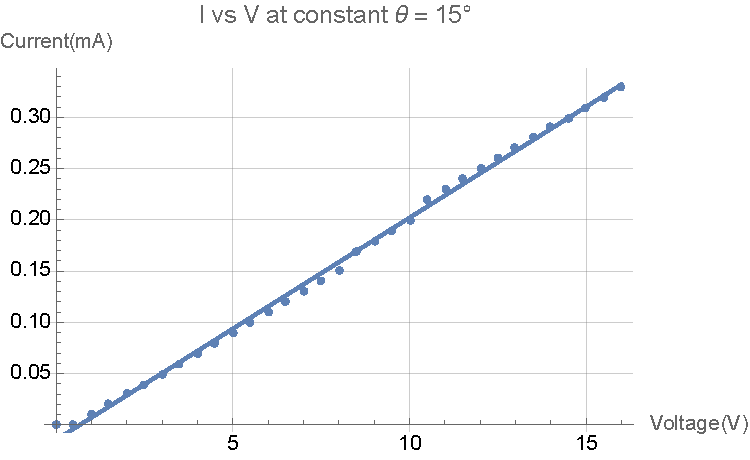
\includegraphics[width=1\textwidth]{graph1} % Include the figure
	\caption{}
\end{figure}
\[
	\boxed{\mu_{CO_2} = (1.03344 \pm 0.00868246) \times  10^{-5} \frac{K}{pa}}
\]
\subsection{\(\Delta T\) vs \(\Delta P\) for \(N_2\)   }
\begin{center}
	\begin{tabular}{ | m{1cm} | m{3cm}| m{3cm} | } 
		\hline
		S.No	&	\(\Delta P\)	&	\(\Delta T\) \\
		\hline
		1&0&-0.08\\
		2&0.05&-0.06\\
		3&0.1&-0.05\\
		4&0.15&-0.04\\
		5&0.2&-0.03\\
		6&0.25&-0.01\\
		7&0.3&-0.01\\
		8&0.35&0\\
		9&0.4&0.01\\
		10&0.45&0.01\\
		11&0.5&0.02\\
		12&0.55&0.03\\
		13&0.6&0.04\\
		14&0.65&0.06\\
		15&0.7&0.07\\
		16&0.75&0.08\\
		17&0.8&0.1\\
		18&0.85&0.11\\
		19&0.9&0.11\\
		20&0.95&0.12\\
		21&1&0.12\\
		\hline
	\end{tabular}
\end{center}
\begin{figure}[H] % [H] forces the figure to be placed exactly where it appears in the text
	\centering % Horizontally center the figure
	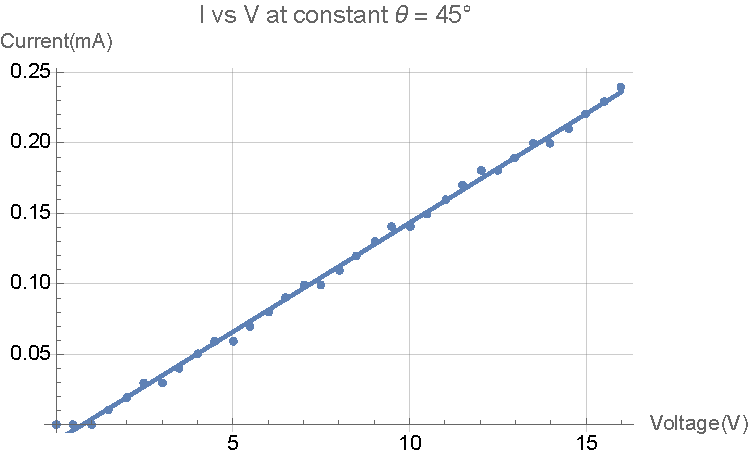
\includegraphics[width=1\textwidth]{graph2} % Include the figure
	\caption{}
\end{figure}
\[
	\boxed{\mu_{N_2} = (0.0201588 \pm 0.00637132 ) \times 10^{-5} \frac{K}{pa}}
\]
\section{Calculations}
\subsection{Theoretical value of Joule-Thomson coefficient of  \(CO_{2}\)}

\begin{gather*}	
	a = 3.60 Pa \frac{m^6}{mol^2}\\
	b = 42.7 \frac{cm^3}{mol}\\
	c_p = 366.1 \frac{J}{mol K}\\
	T = 304 K \text{(At the time of Experiment)}\\
	\mu_{CO_2} = \left(\frac{2a}{RT} - b\right). \frac{1}{c_p}\\
	\boxed{\mu_{CO_2} = 0.766 \times 10^{-5} \frac{K}{pa}}
\end{gather*}
\subsection{Experimental value of Joule-Thomson coefficient of \(CO_2\)}

\[
	\boxed{\mu_{CO_2} = (1.03344 \pm 0.00868246) \times  10^{-5} \frac{K}{pa}}
\]

\subsection{Theoretical value of Joule-Thomson coefficient of \(N_{2}\)}

\begin{gather*}	
	a =  1.41 Pa \frac{m^6}{mol^2}\\
	b =  39.1 \frac{cm^3}{mol}\\
	c_p = 288.9 \frac{J}{mol K}\\
	T = 304 K \text{(At the time of Experiment)}\\
	\mu_{N_2} = \left(\frac{2a}{RT} - b\right). \frac{1}{c_p}\\
	\boxed{\mu_{N_2} = 0.3699 \times 10^{-5} \frac{K}{pa}}
\end{gather*}

\subsection{Experimental value of Joule-Thomson coefficient of \(N_2\)}

\[
	\boxed{\mu_{N_2} = (0.0201588 \pm 0.00637132 ) \times 10^{-5} \frac{K}{pa}}	
\]

\section{Conclusion}
The literature values are 
\[
	\mu_{CO_2} = 1.16 \times 10^{-5} \frac{K}{Pa} 
\]
at \(20^{\circ}C\) and $10^{5}$ pa
\[
	\mu_{N_2} = 0.23 \times 10^{-5} \frac{K}{Pa}
\]
at \(20^{\circ}C\) and $10^{5}$ pa. \\

The experimental values are 

\[
	\boxed{\mu_{CO_2} = (1.03344 \pm 0.00868246) \times  10^{-5} \frac{K}{pa}}
\]
at \(31 ^{\circ}\)C and \(10^5\) pa.
\[
	\boxed{\mu_{N_2} = (0.0201588 \pm 0.00637132 ) \times 10^{-5} \frac{K}{pa}}	
\]
at \(31 ^{\circ}\)C and \(10^5\) pa. 
The literature values and experimental values are in the limit of error.
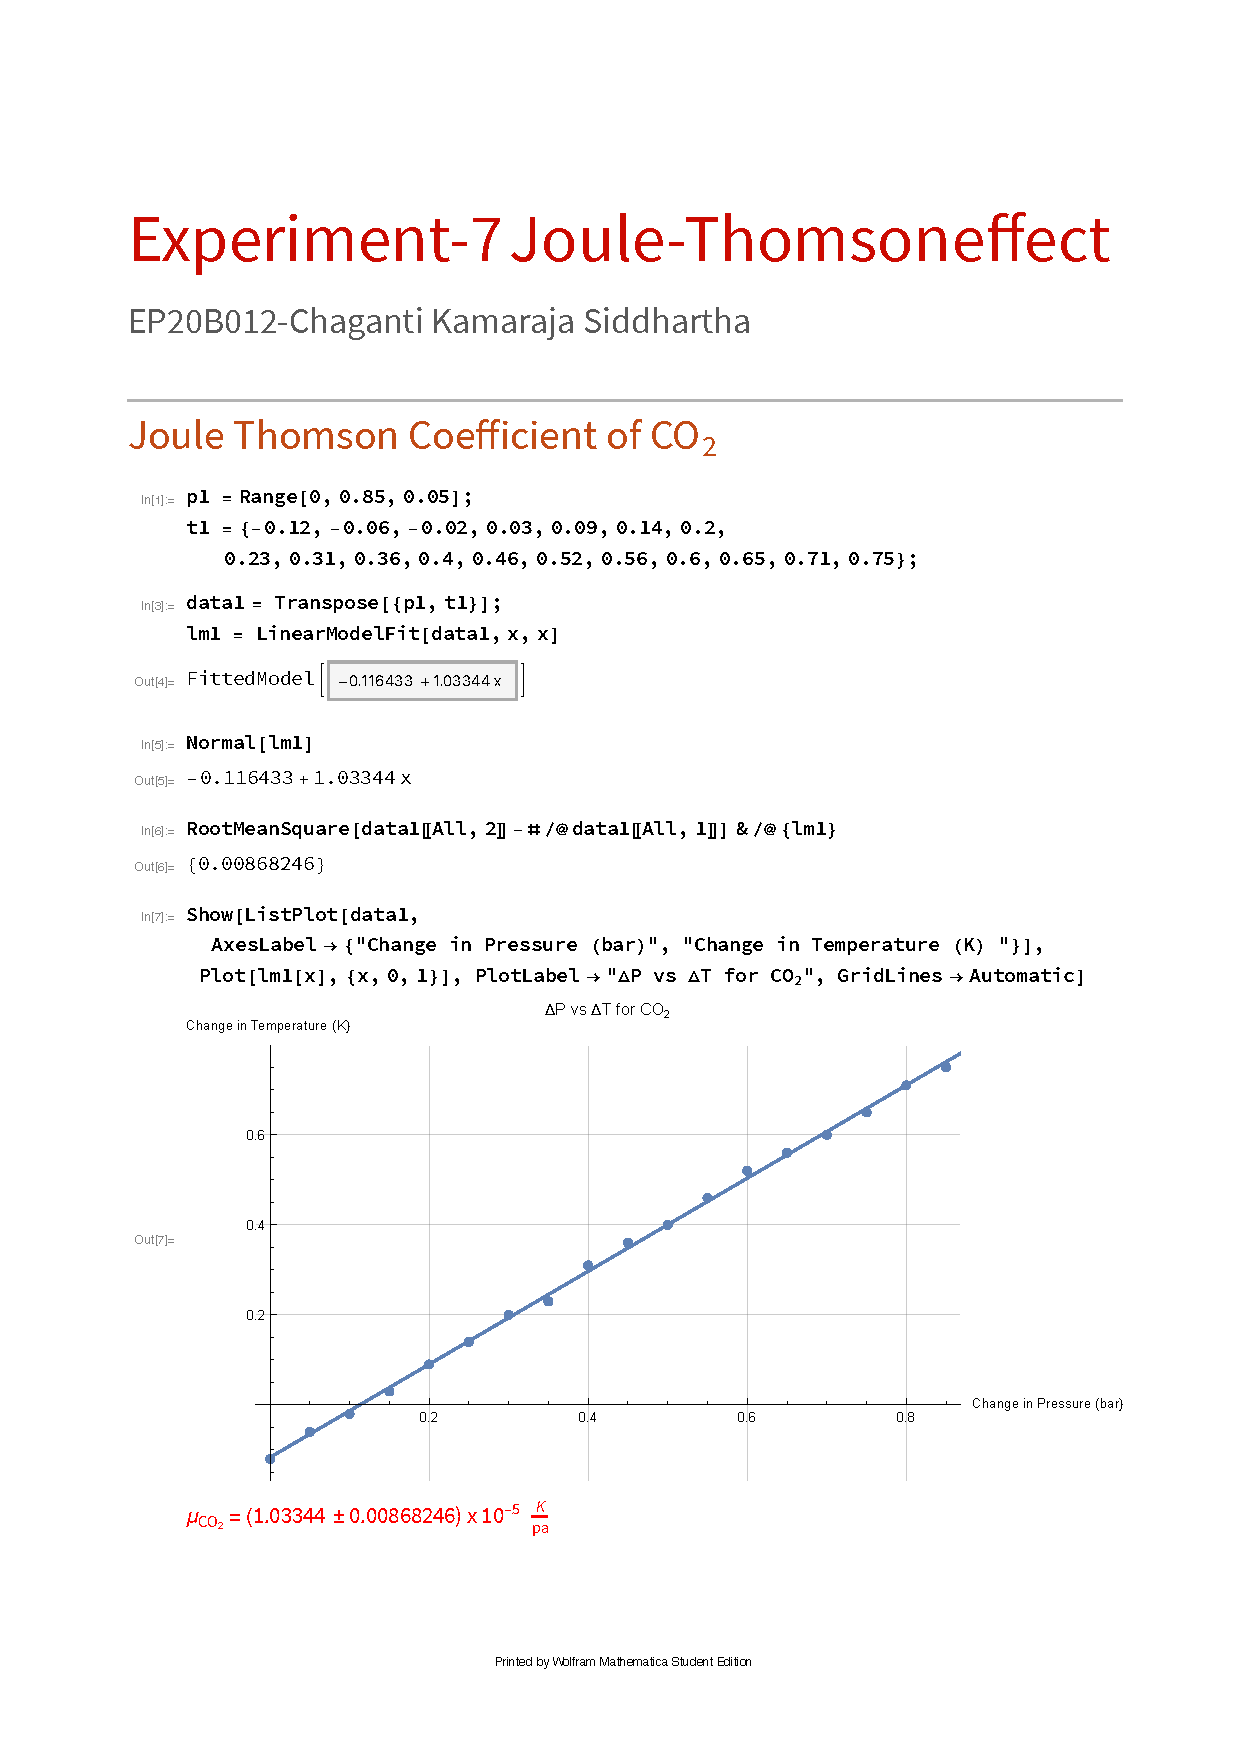
\includepdf[pages=-]{Exp7.pdf}
\end{document}
